\chapter{Technik/Methoden}
\label{cha:Technik}

\section{Stand der Technik}
\label{sec:Stand der Technik}

\subsection{Propan in Kälteanlagen}
\label{subsec:Propan in Kälteanlagen}

\subsection{Normalkühlung}
\label{subsec:Normalkühlung}

\subsection{Komponenten einer Kälteanlage}
\label{subsec:Komponenten einer Kälteanlage}

\section{Das Kühlregal}
\label{sec:Das Kühlregal}

Der Mittelpunkt der durchgeführten Untersuchungen ist ein vertikales Verkaufskühlmöbel der Firma AHT.
Es umfasst auf einer Länge von \unit{3,75}{\metre} vier Regalböden um Produkte zu kühlen und auszustellen. Ein von oben herabfallender Luftschleier ermöglicht ein türloses Design des Regals. Die Kälteerzeugung wird, wie in Abbildung~\ref{fig:IDC150} ersichtlich, durch drei seperate Kältekreisläufe gewährleistet. Das verwendete Kältemittel ist Propan (R290). Jeder Kreis besitzt eine Füllmenge von \unit{150}{\gram}. Um die Füllmenge zu reduzieren wurden bereits vor Beginn der Untersuchungen kältetechnische Komponenten mit geringerem internen Volumen eingebaut. Die Verdichter sind ein Produkt der Firma Emerson. Im Rahmen der Untersuchungen kommen mehrere Modelle zum Einsatz. Drei Plattenwärmeübertrager der Firma SWEP dienen als Verflüssiger. Sie besitzen je 20 Platten und eine Nennleistung von je \unit{2,7}{\kilo\watt}. Die Expansionsventile der Firma Alco sind elektronisch regelbar und besitzen einen Temperatur- sowie Drucksensor in der Saugleitung. Die drei Kreisläufe durchlaufen mit je sechs Durchgängen einen gemeinsamen Verdampfer dessen Lamellenabstand \unit{5}{\milli\metre} beträgt. Sechs Lüftermotoren der Firma EBM Pabst saugen die Luft durch den Verdampfer mit einer konstanten Drehzahl von \unit{1400}{U\per\min}.

\begin{figure} %[!htb]
\centering
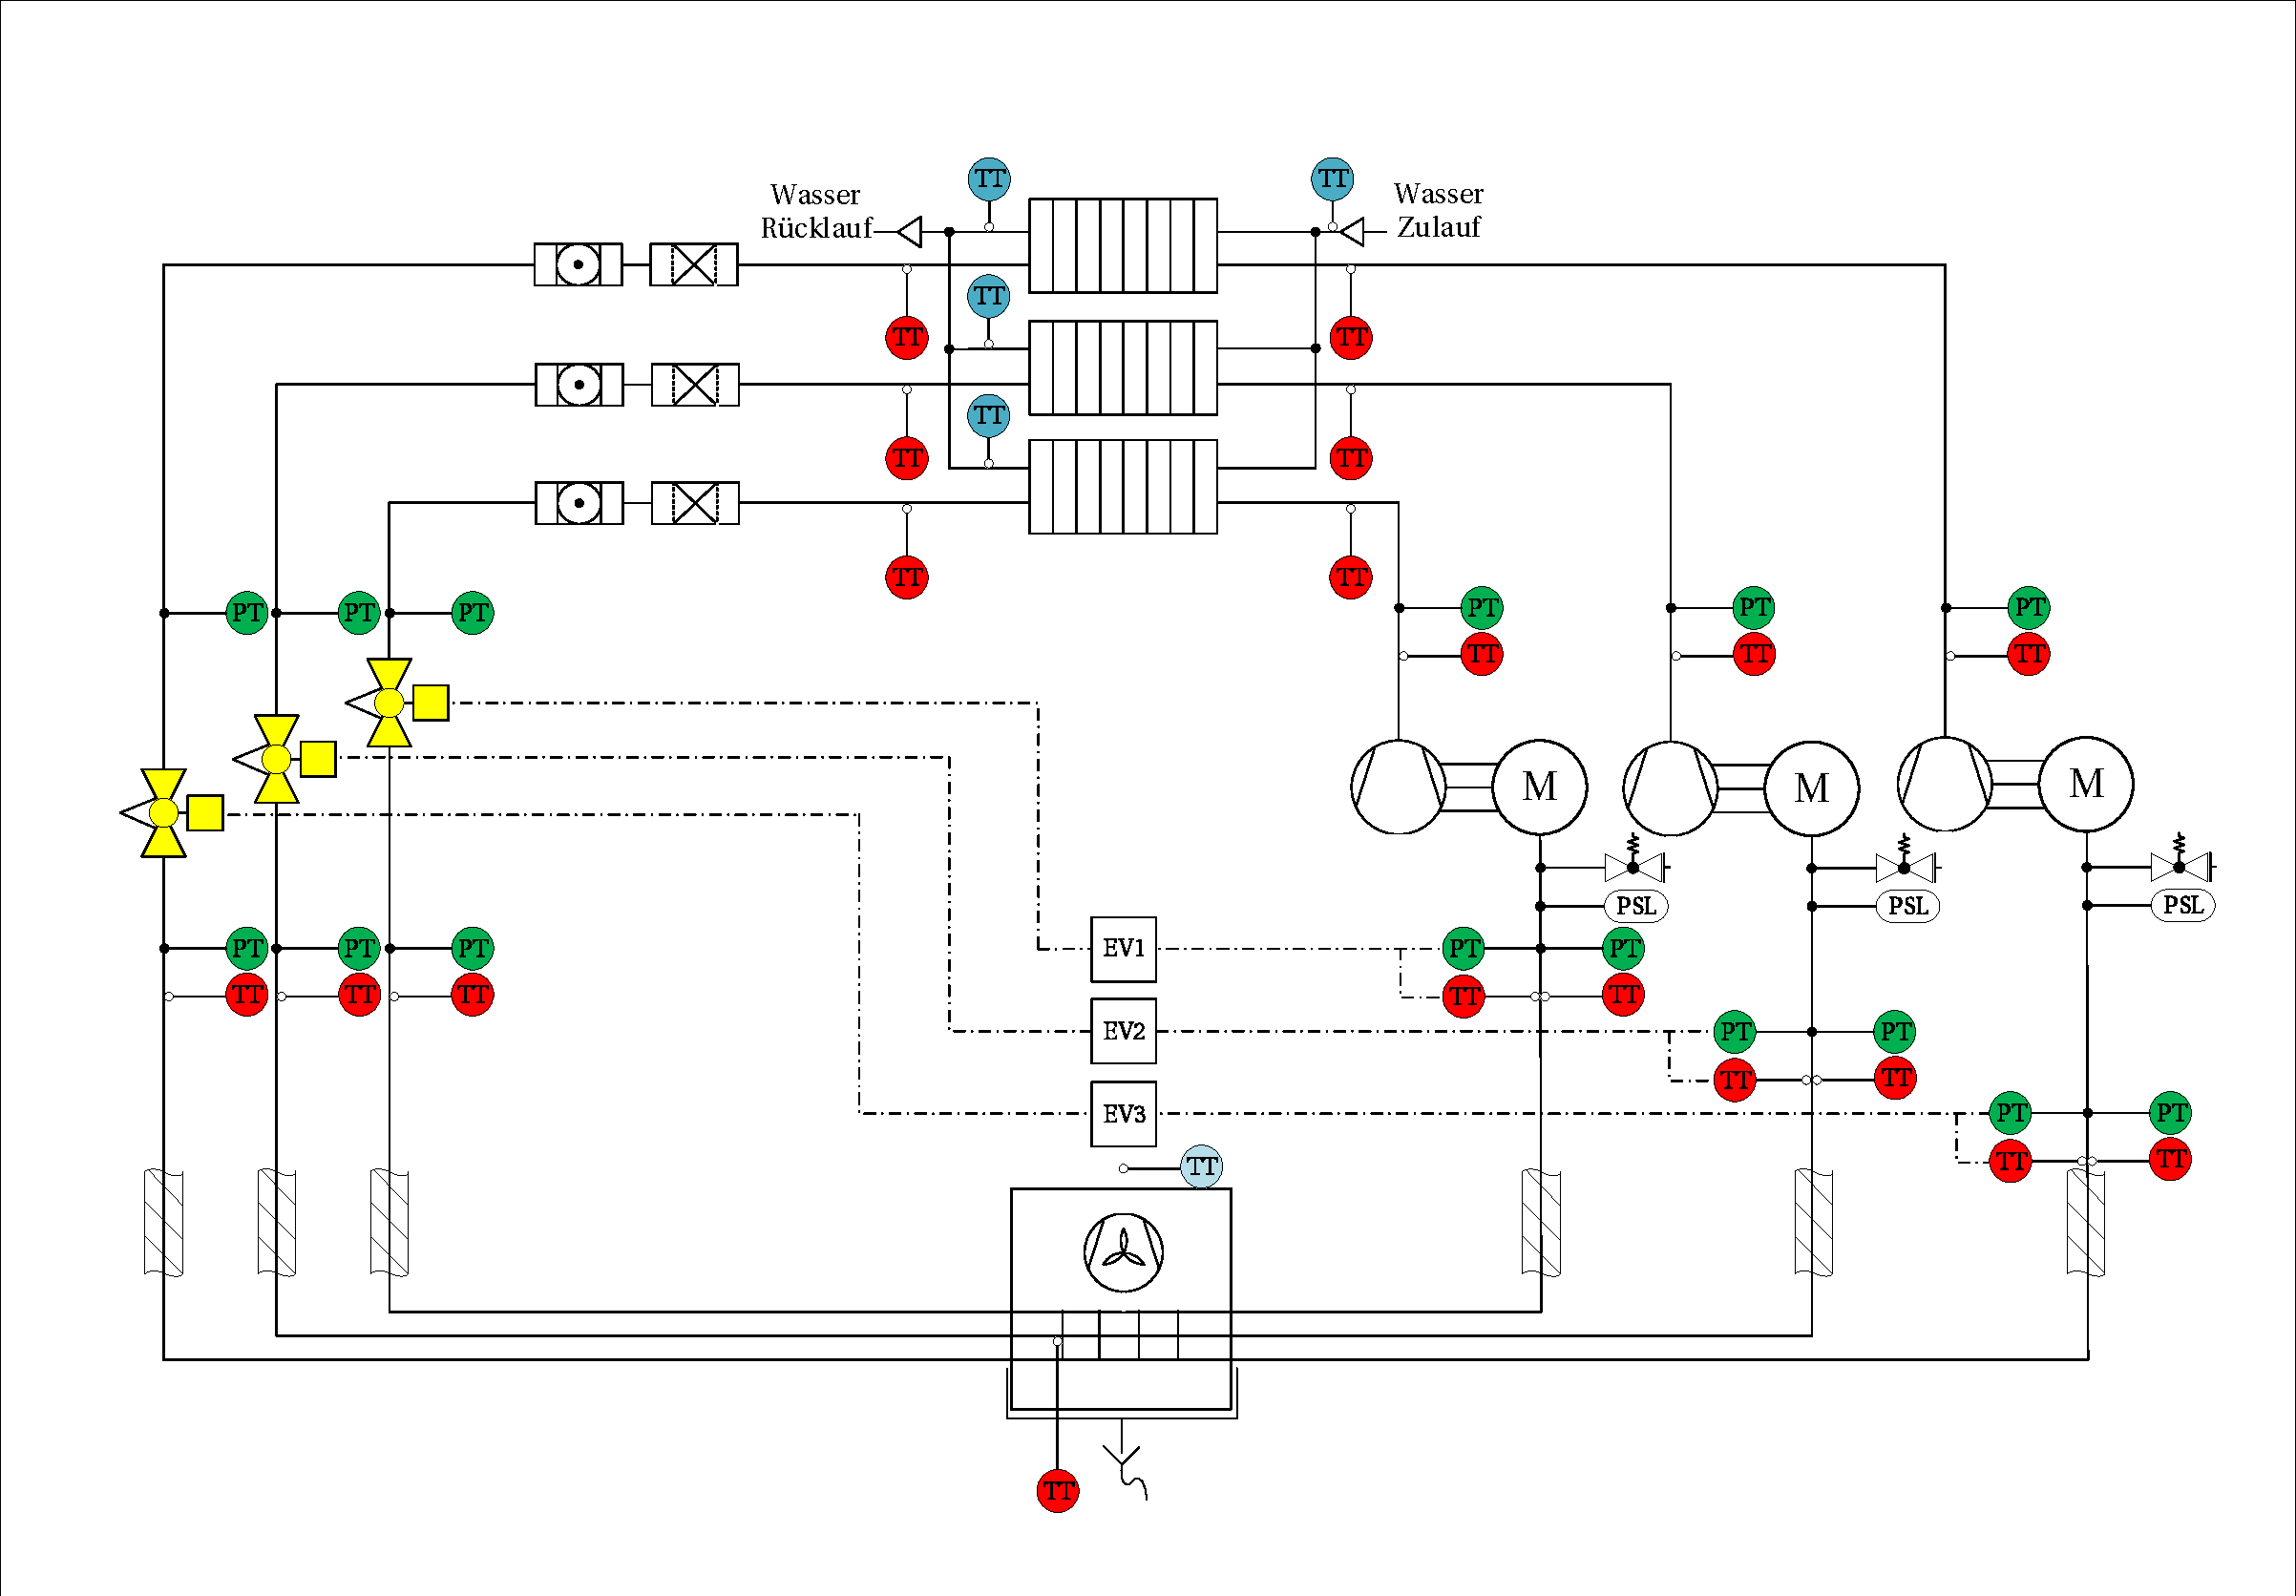
\includegraphics[scale=.5,angle=90]{Pictures/IDC150.pdf}
\caption{Kältekreise des Kühlmöbels}
\label{fig:IDC150}
\end{figure}


\section{Die Klimakammer}
\label{sec:Die Klimakammer}

Um während den Untersuchungen gleichbleibende Umgebungsbedingungen zu generieren und so reproduzierbare Ergebnisse zu erzielen, steht das Kühlregal in einer Klimakammer.
Wie in Abbildung~\ref{fig:Klimakammer} zu erkennen besteht die Klimakammer eigentlich aus zwei kleineren Kammern mit eigenständigen Zuluftregelungen. Aufgrund der Größe des Regals wurde die Trennwand zwischen den Kammern entfernt. Die Zuluftaufbereitung übernimmt dabei die Klimaanlage der Kammer B. Damit die aufbereitete Luft den Raum über seine gesamte Länge durchströmt wurde die Ansaugöffnung von Kammer B mit einer Decke, die bis zum Ende des Raums reicht, abgedeckt. Vor den Luftauslassgittern besitzen die Kammern Umlenkbleche. Diese sollen eine gleichmäßige Verteilung des Luftmassenstroms über den Austrittquerschnitt erzielen. Die Klimaanlagen sind in der Lage die angesaugte Raumluft zu kühlen, aufzuheizen, sowie zu be- und entfeuchten. Die Regelung findet dabei über einen Computer statt. Mithilfe von LabView, welches eine intuitive Benutzeroberfläche bietet, lässt sich Einfluss auf die Soll-Werte, die Dauer der jeweiligen Untersuchung und die Einstellung der Regelparameter nehmen. 
Jede Kammer besitzt zudem einen Wasseranschluss dessen Vorlauftemperatur regulierbar ist.
Die Verflüssiger des Kühlregals werden mit temperiertem Wasser der Regelung von Kammer A beaufschlagt. 


\begin{figure}[htb]
\centering
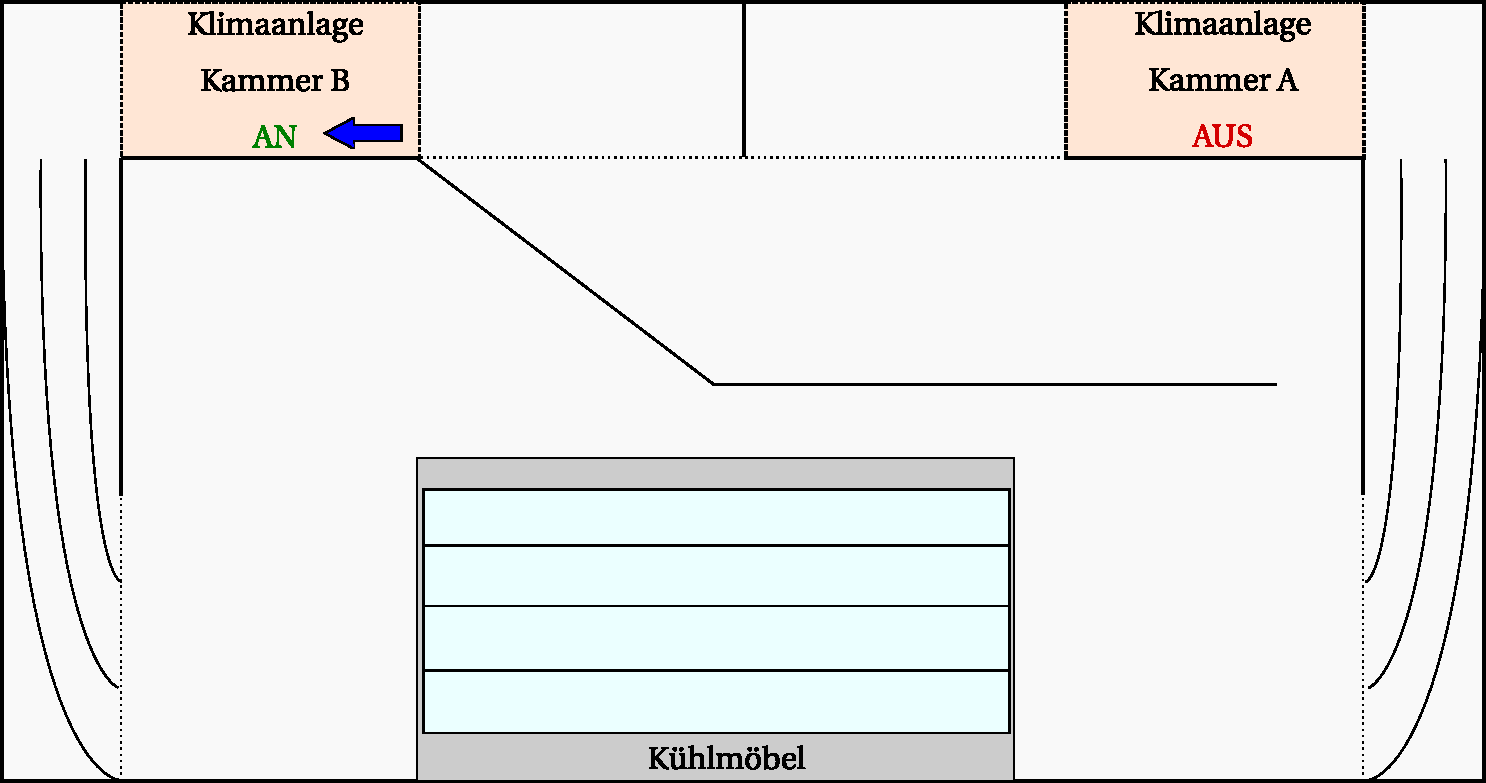
\includegraphics[scale=.5]{Pictures/ClimateChamber.pdf}
\caption{Klimakammer}
\label{fig:Klimakammer}
\end{figure}

\section{Erfassung von Messdaten}
\label{sec:Erfassung von Messdaten}

Um alle physikalischen Größen während des Betriebs möglichst genau zu erfassen und zu speichern werden entsprechende Geräte und Programme eingesetzt. Insgesamt finden drei Systeme Anwendung um sensorbasiert Daten zu erfassen, umzuwandeln und in Tabellenform zu speichern.

\subsection{Messdaten der Klimakammer}
\label{subsec:Messdaten der Klimakammer}

Die in Abschnitt~\ref{sec:Die Klimakammer} vorgestellte Klimakammer wird über LabView gesteuert. Die erfassten Messdaten sind raumluftseitig Ist- und Mittelwerte der Temperaturen sowie die relative Luftfeuchtigkeit. Wasserseitig werden Wassermassenstrom sowie Vor- und Rücklauftemperatur gemessen. 
Die Sensoren, welche die Regelgrößen Temperatur und relative Luftfeuchtigkeit aufnehmen, sind zuluftseitig in der Nähe des Auslassgitters positioniert. Die Regelgröße der Temperatur entspricht dem Mittelwert von drei, über die Höhe des Luftauslassgitters verteilten Temperatursensoren. Wird der Betrieb der Klimakammer über das Programm gestartet so wird eine Exceldatei erstellt in die in einem Intervall von \unit{1}{\second} die erfassten Daten geschrieben werden.


\subsection{Messdaten des Kühlregals}
\label{subsec:Messdaten der Klimakammer}

Mithilfe des Programms NI SignalExpress werden die Messdaten des Kühlregals und der Kältekreisläufe via Modbus erfasst. Um die Temperaturen zu messen werden Thermoelemente  und um die Drücke zu messen Hochgenauigkeitsdruckaufnehmer verwendet. Die erfassten Messwerte sind die Produkttemperaturen sowie Ein- und Austrittstemperatur der Luft am Verdampfer des Kühlregals, die Temperaturen an verschiedenen Positionen der Kältekreisläufe und die Relativdrücke des Kältemittels im System in Heißgasleitung, Flüssigkeitsleitung, Einspritzleitung und Saugleitung. Die Positionen der Sensoren an den Kältekreisläufen sind aus Abbildung~\ref{fig:IDC150} ersichtlich. Zudem wurde noch die Temperatur des Kältemittels nach jedem einzelnen Durchgang durch den Verdampfer erfasst.
In einem Intervall von \unit{5}{\second} werden die erfassten Daten in eine Exceltabelle geschrieben. SignalExpress erstellt in Echtzeit Graphen der Messwerte. Somit lässt sich das Verhalten des Systems jederzeit beobachten.

\subsection{Messdaten des Leistungsanalysators}
\label{subsec:Messdaten des Leistungsanalysators}

Um den Zustand des Systems auch elektroseitig zu erfassen wird ein Yokogawa WT3000 Leistungsanalysator verwendet. Dieser ist in der Lage Spannungen, Ströme mit einer Genauigkeit von \unit{0,02}{\%} zu erfassen und daraus Blind-, Wirk- und Scheinleistungen zu berechnen. Die abgenommenen Komponenten sind die einzelnen Verdichter, die Ventilatoren und die restlichen Verbraucher des Kühlregals, wie Licht und Relays.
Das Gerät speichert die erfassten und berechneten Messwerte in Tabellenform auf einem externen Datenspeicher. Die Intevalllänge beträgt hierbei \unit{5}{\second}.


\section{Testbedingungen nach Norm}
\label{sec:Testbedingungen nach Norm}

Die Norm DIN EN ISO 23953-2 liefert Vorgaben zum Aufbau des Prüfstandes, zur Position der Messtechnik und zu Berechnungsmethoden. Bei allen Tätigkeiten wurde sich an dieser orientiert um reproduzierbare sowie vergleichbare Ergebnisse zu erzielen. Rahmenbedingung ist, dass alle Untersuchungen, nach Tabelle~\ref{tab:Klimaklassen}, bei Klimaklasse 3 durchgeführt werden. Die erzielten Produkttemperaturen des Kühlmöbels müssen dabei, gemäß Tabelle~\ref{tab:Temperaturklassen}, zwischen \unit{5}{\celsius} und \unit{-1}{\celsius} liegen.
Um Kühlgut möglichst genau zu simulieren, werden je \unit{1}{\kilogram} schwere M-Pakete aus Silikon verwendet.
Diese werden entsprechend Abbildung~\ref{fig:Anordnung der M-Pakete} positioniert und jene die mit einem X gekennzeichnet sind mit Temperatursensoren versehen.
Der Messpunkt für die Temperatur und die relative Luftfeuchte muss mittig der Länge der Kühlmöbels und \unit{300}{\milli\metre} vor dessen Oberkante liegen.
Voraussetzung für eine normgerechte Messung ist zudem, dass eine Bewegung der Luft vorhanden ist. Deren Geschwindigkeit muss an den drei Messpunkten auf der Linie A-A in Abbildung~\ref{fig:Messpunkte} zwischen \unit{0,1}{\meter\per\second} und \unit{0,2}{\meter\per\second} liegen\cite{DINDeutschesInstitutfurNormunge.V..}.







% Please add the following required packages to your document preamble:
% \usepackage[table,xcdraw]{xcolor}
% If you use beamer only pass "xcolor=table" option, i.e. \documentclass[xcolor=table]{beamer}
\begin{table}[h!]
\centering
\caption{Klimaklassen~\cite{DINDeutschesInstitutfurNormunge.V..}}
\label{tab:Klimaklassen}
\begin{tabular}{|c|c|c|c|c|}
\hline
\textbf{\begin{tabular}[c]{@{}c@{}}Klimaklasse des \\ Prüfraums\end{tabular}} & \textbf{\begin{tabular}[c]{@{}c@{}}Trockenkugel-\\ temperatur\end{tabular}} & \textbf{\begin{tabular}[c]{@{}c@{}}Relative \\ Luftfeuchte\end{tabular}} & \textbf{Taupunkt} & \textbf{\begin{tabular}[c]{@{}c@{}}Wasserdampf-\\ gehalt \\ in trockener Luft\end{tabular}} \\
                                                                              &                                                                             & \%                                                                       & °C                & g/kg                                                                                        \\ \hline
0                                                                             & 20                                                                          & 50                                                                       & 9,3               & 7,3                                                                                         \\ \hline
1                                                                             & 16                                                                          & 80                                                                       & 12,6              & 9,1                                                                                         \\ \hline
8                                                                             & 23,9                                                                        & 55                                                                       & 14,3              & 10,2                                                                                        \\ \hline
2                                                                             & 22                                                                          & 65                                                                       & 15,2              & 10,8                                                                                        \\ \hline
\rowcolor[HTML]{FFFe65}
3                                                                             & 25                                                                          & 60                                                                       & 16,7              & 12                                                                                          
\\ \hline
4                                                                             & 30                                                                          & 55                                                                       & 20                & 14,8                                                                                        \\ \hline
5                                                                             & 27                                                                          & 70                                                                       & 21,1              & 15,8                                                                                        \\ \hline
6                                                                             & 40                                                                          & 40                                                                       & 23,9              & 18,8                                                                                        \\ \hline
7                                                                             & 35                                                                          & 75                                                                       & 30                & 27,3                                                                                        \\ \hline
\end{tabular}
\end{table}

\begin{figure}[h!tb]
\centering
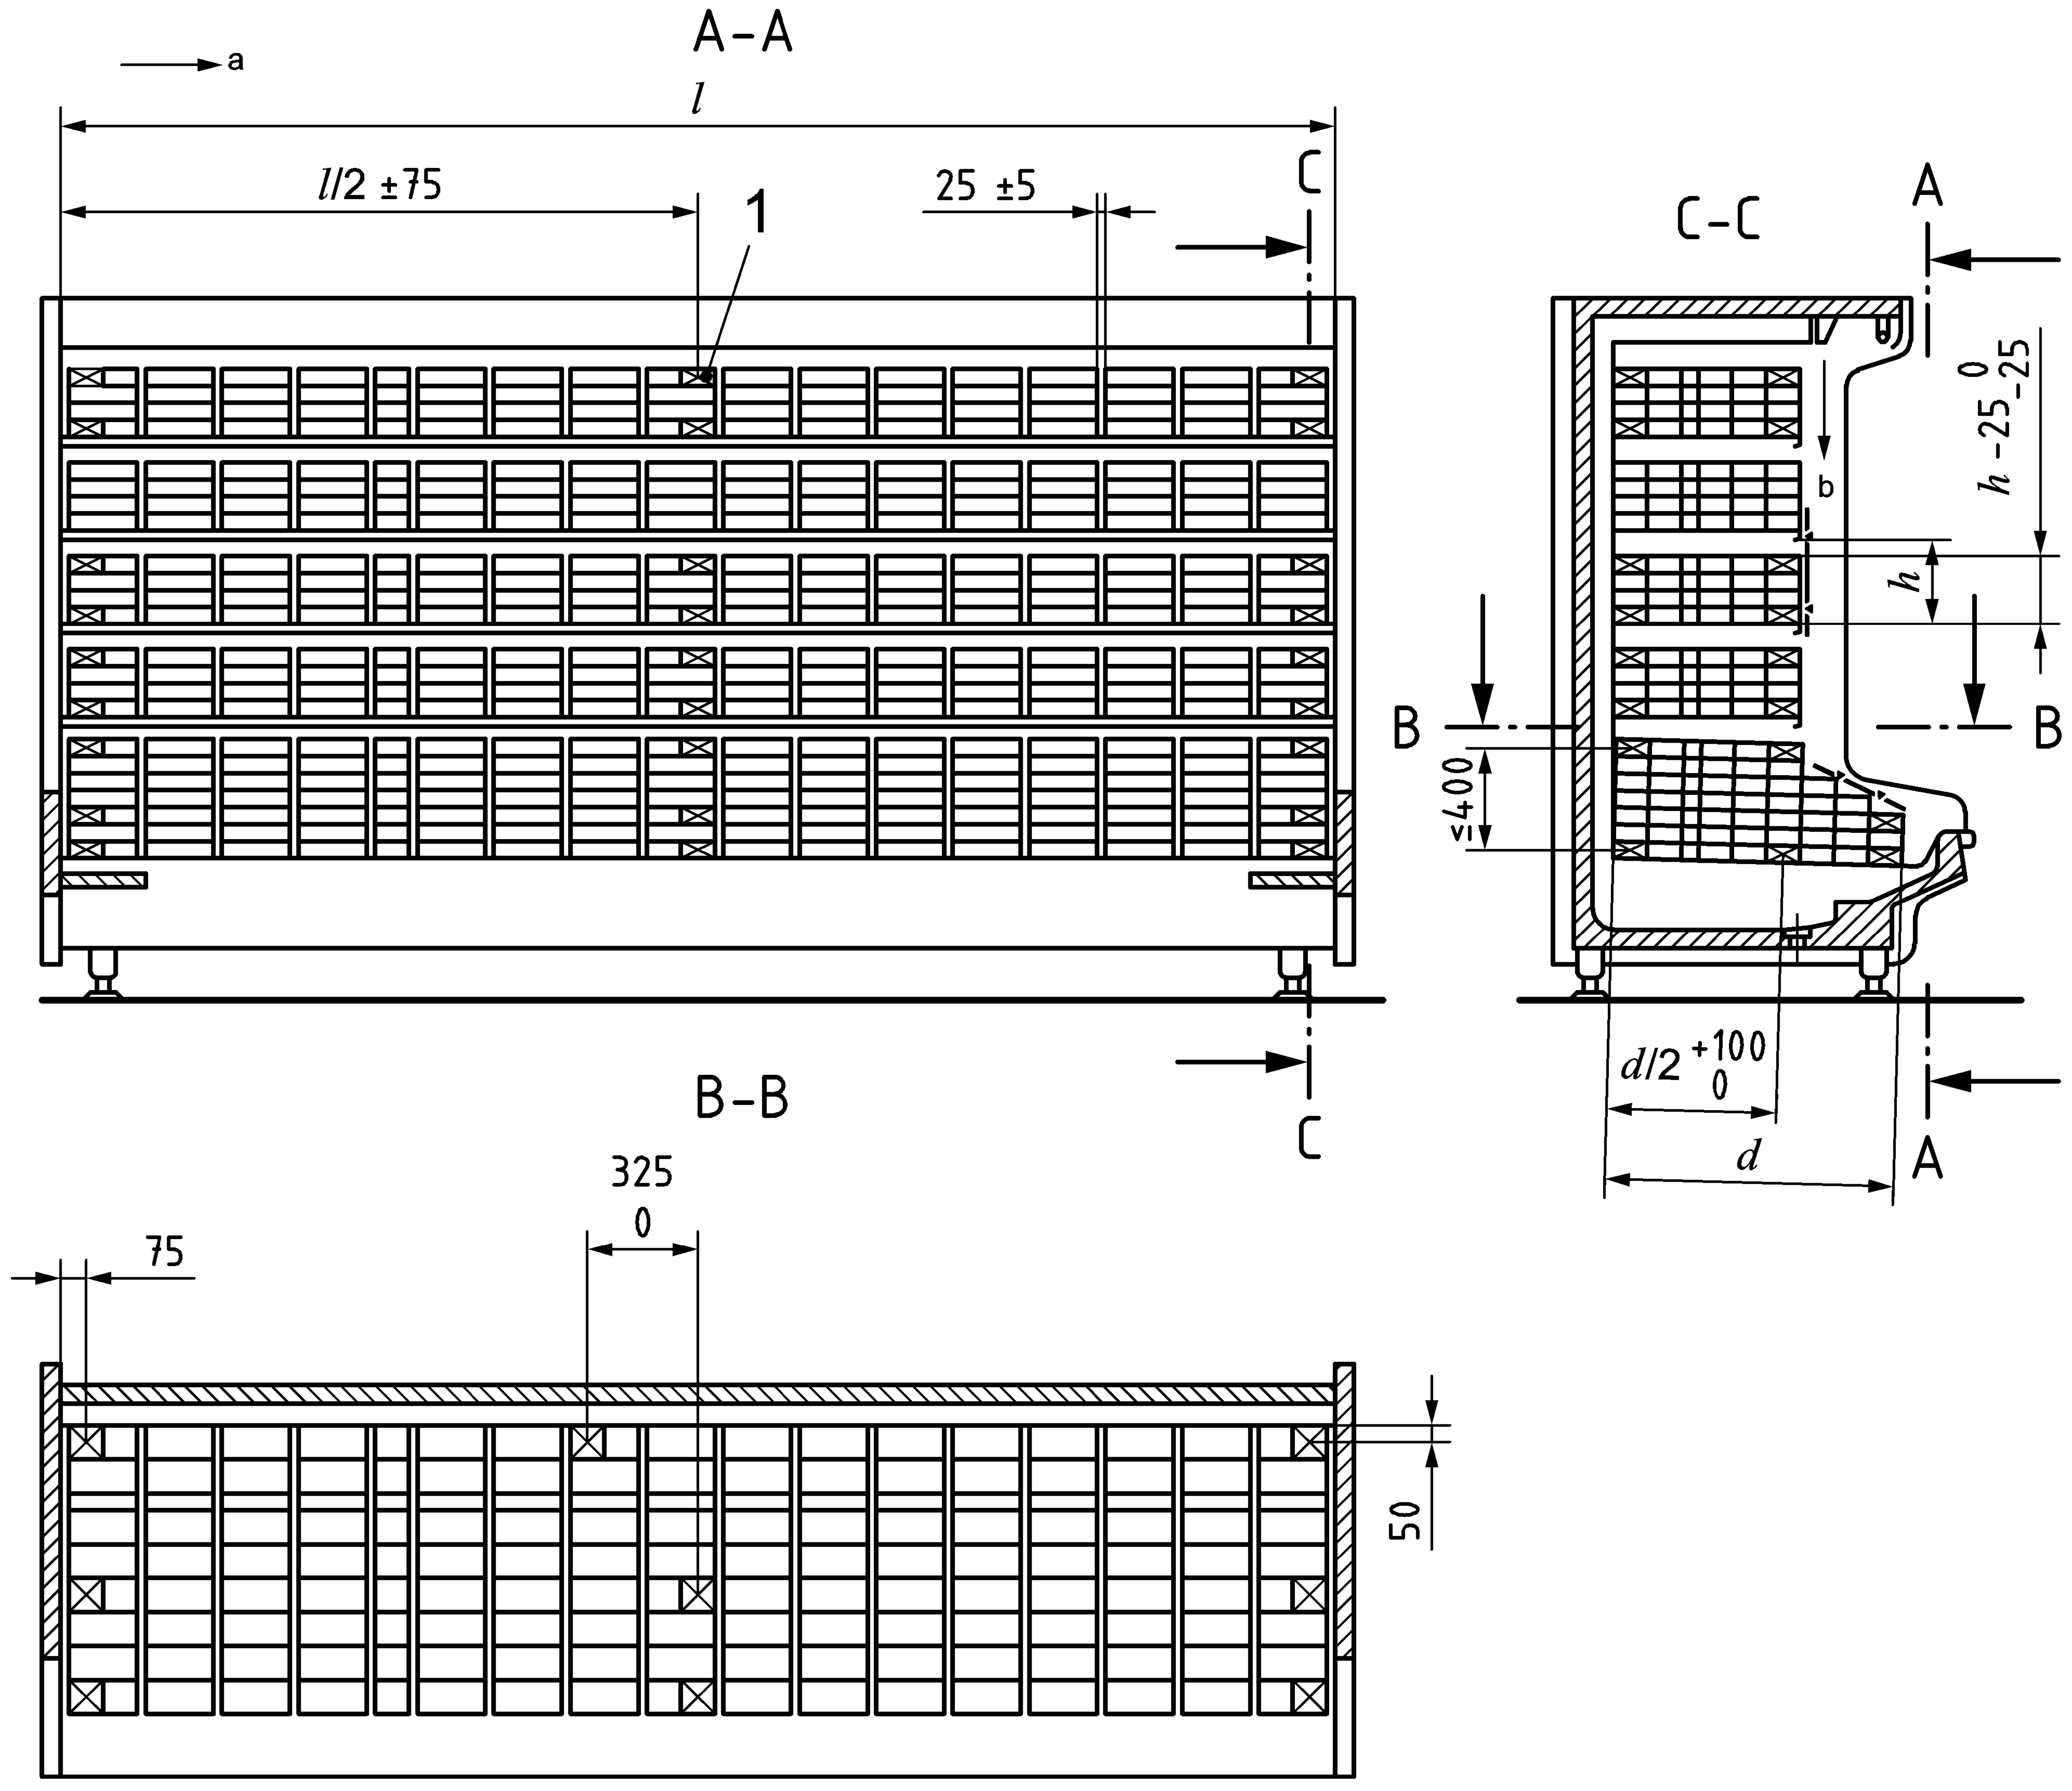
\includegraphics[scale=.12]{Pictures/multi-deck-chilled-cabinet.pdf}
\caption{Anordnung der M-Pakete und der Temperatursensoren~\cite{DINDeutschesInstitutfurNormunge.V..}}
\label{fig:Anordnung der M-Pakete}
\end{figure}

% Please add the following required packages to your document preamble:
% \usepackage[table,xcdraw]{xcolor}
% If you use beamer only pass "xcolor=table" option, i.e. \documentclass[xcolor=table]{beamer}
\begin{table}[h!]
\centering
\caption{Temperaturklassen der M-Pakete~\cite{DINDeutschesInstitutfurNormunge.V..}}
\label{tab:Temperaturklassen}
\begin{tabular}{|c|c|c|}
\hline
\textbf{Klasse} & \textbf{\begin{tabular}[c]{@{}c@{}}Höchste Temperatur,\\ des wärmsten\\ M-Pakets gleich oder\\ niedriger als\end{tabular}} & \textbf{\begin{tabular}[c]{@{}c@{}}Niedrigste Temperatur,\\ des kältesten\\ M-Pakets gleich oder\\ höher als\end{tabular}} \\ \cline{2-3} 
                & \multicolumn{2}{c|}{°C}                                                                                                                                                                                                                                 \\ \hline
L1              & -15                                                                                                                        & -                                                                                                                          \\ \hline
L2              & -12                                                                                                                        & -                                                                                                                          \\ \hline
L3              & -12                                                                                                                        & -                                                                                                                          \\ \hline
\rowcolor[HTML]{FFFE65} 
M1              & +5                                                                                                                         & -1                                                                                                                         \\ \hline
M2              & +7                                                                                                                         & -1                                                                                                                         \\ \hline
H1              & +10                                                                                                                        & +1                                                                                                                         \\ \hline
H2              & +10                                                                                                                        & -1                                                                                                                         \\ \hline
S               & \multicolumn{2}{c|}{Sonderklasse}                                                                                                                                                                                                                       \\ \hline
\end{tabular}
\end{table}




\begin{figure}[h!tb]
\centering
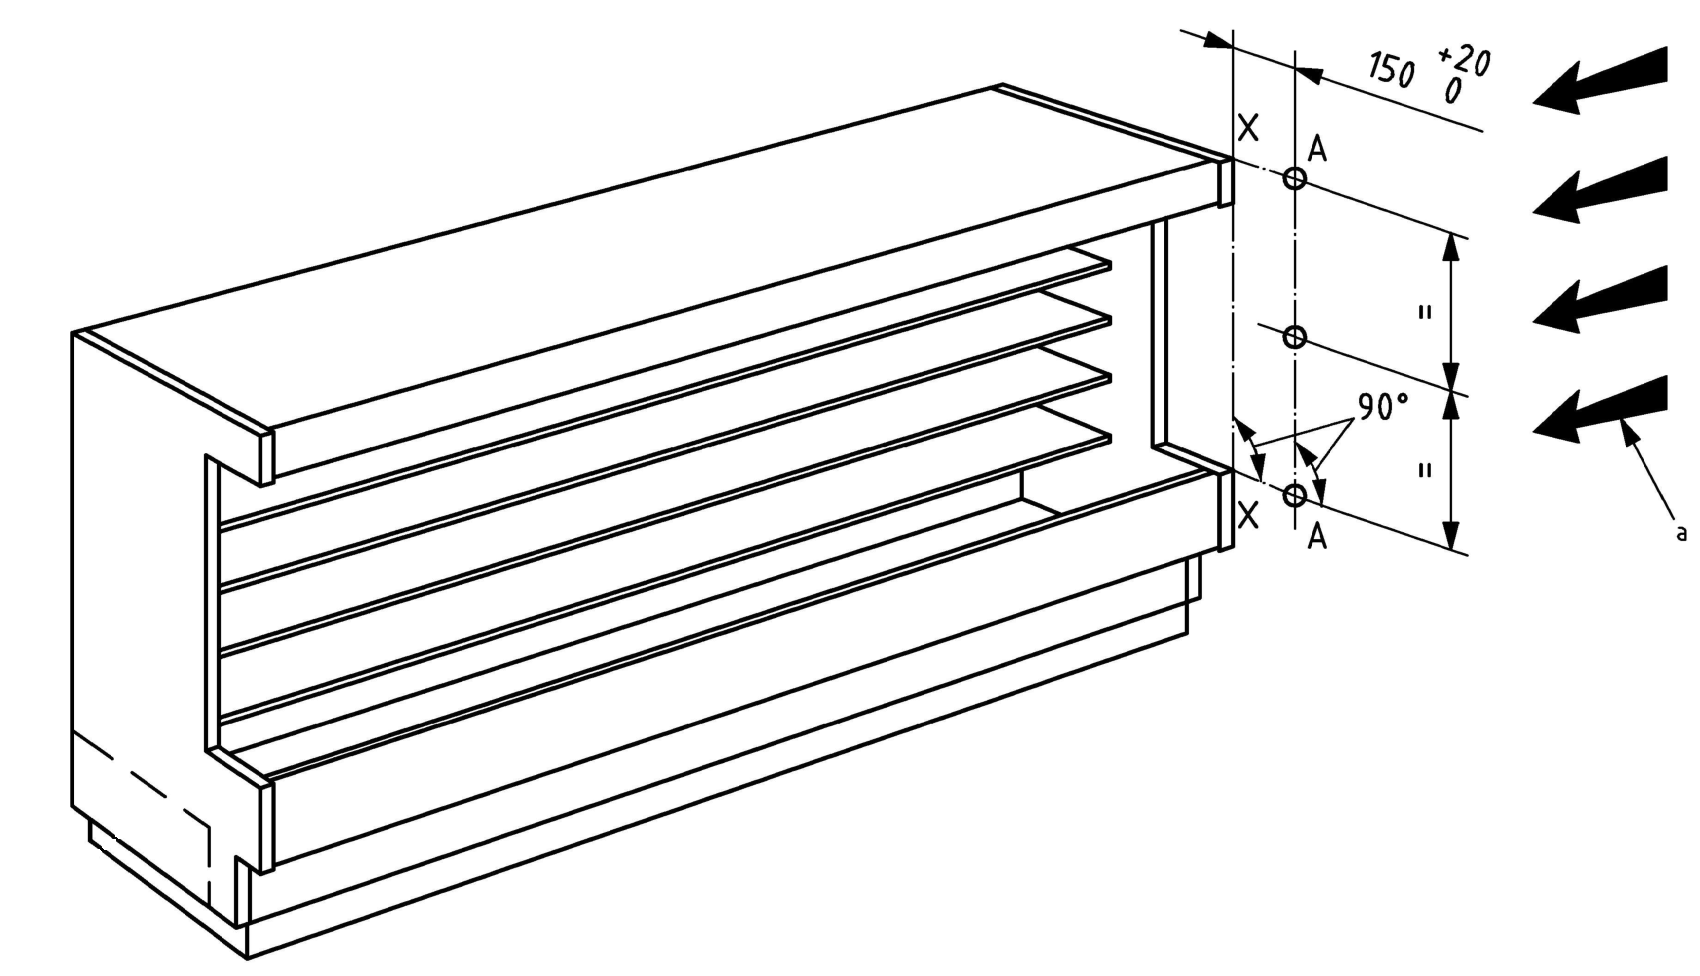
\includegraphics[scale=.5]{Pictures/idc_meas.pdf}
\caption{Messpunkte~\cite{DINDeutschesInstitutfurNormunge.V..}}
\label{fig:Messpunkte}
\end{figure}


\section{Simulationsmodell für Verschaltung der Verdampferrohre}
\label{sec:Simulationsmodell}

Mithilfe des Programms EES (Engineering Equation Solver) wurde im Rahmen der Untersuchungen ein Modell erstellt, welches es ermöglicht den Effekt einer anderen Verschaltung der kältemittelführenden Leitungen innerhalb des Verdampfers auf dessen Kälteleistung zu simulieren. Grundidee hinter dem Modell ist den, durch den hohen Kältemittelmassenstrom bei gleichzeitig geringem Durchmesser der Verdampferrohre bedingten, Druckabfall und das damit einhergehende Absinken der Sättigungstemperatur zur Erhöhung der Kälteleistung zu nutzen. Im Ausgangsmodell durchströmt das Kältemittel den Verdampfer im Gegenstromprinzip. Aufgrund des Druckabfalls verhält sich diese Anordung wie eine Kombination aus Gleich- und Gegenstrom. Wird nun die Anordnung der Rohre dahingehend geändert, dass das Kältemittel den Verdampfer von dessen Mitte aus im Gleichstrom mit der Luft nach oben durchströmt, aber die überhitzten Rohrreihen noch immer beim Lufteintritt sind, so erzielt man den gegenteiligen Effekt: Der Wärmeübertrager bietet eine Kombination aus Gleich- und Gegenstrom, verhält sich aber wie ein reiner Gegenstromverdampfer. Hierbei ist am Verdampferaustritt der Luft eine höhere Temperaturdifferenz zum Kältemittel zu erwarten. Den Vergleich zeigt Abbildung~\ref{fig:Vergleich der Verdampferschaltungen}.
Das Modell soll zeigen ob diese Maßnahme einen bedeutenden Effekt erzielen kann und wird anschließend im Versuch validiert.


\begin{figure}[htb]
\centering
	\subfigure[Ausgangsschaltung]{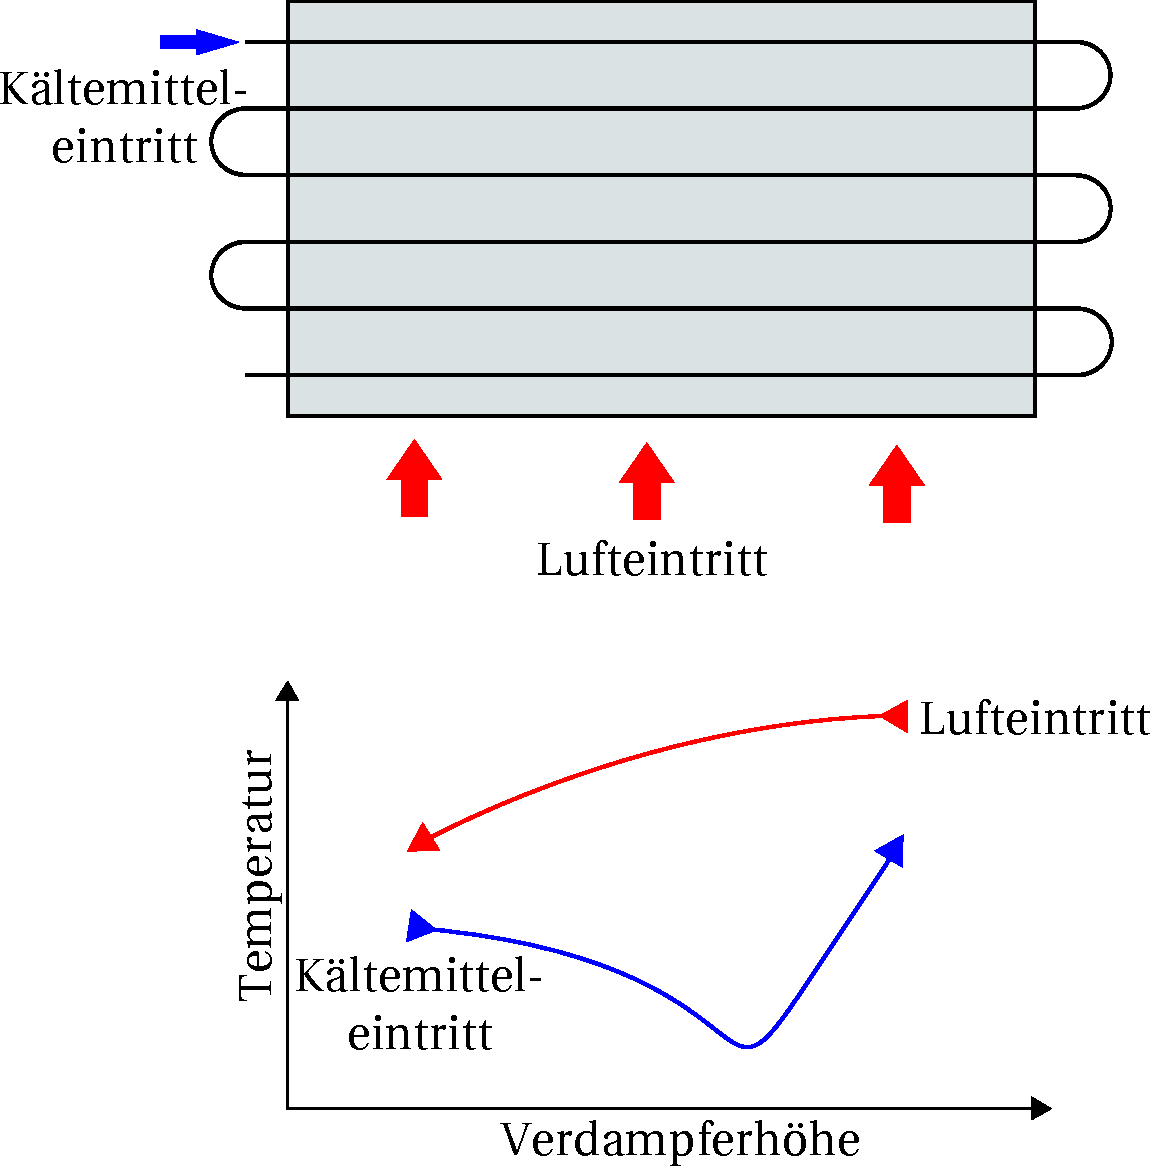
\includegraphics[scale=0.4]{Pictures/Verdampfer_Gegenstrom.pdf}}
	\subfigure[veränderte Schaltung]{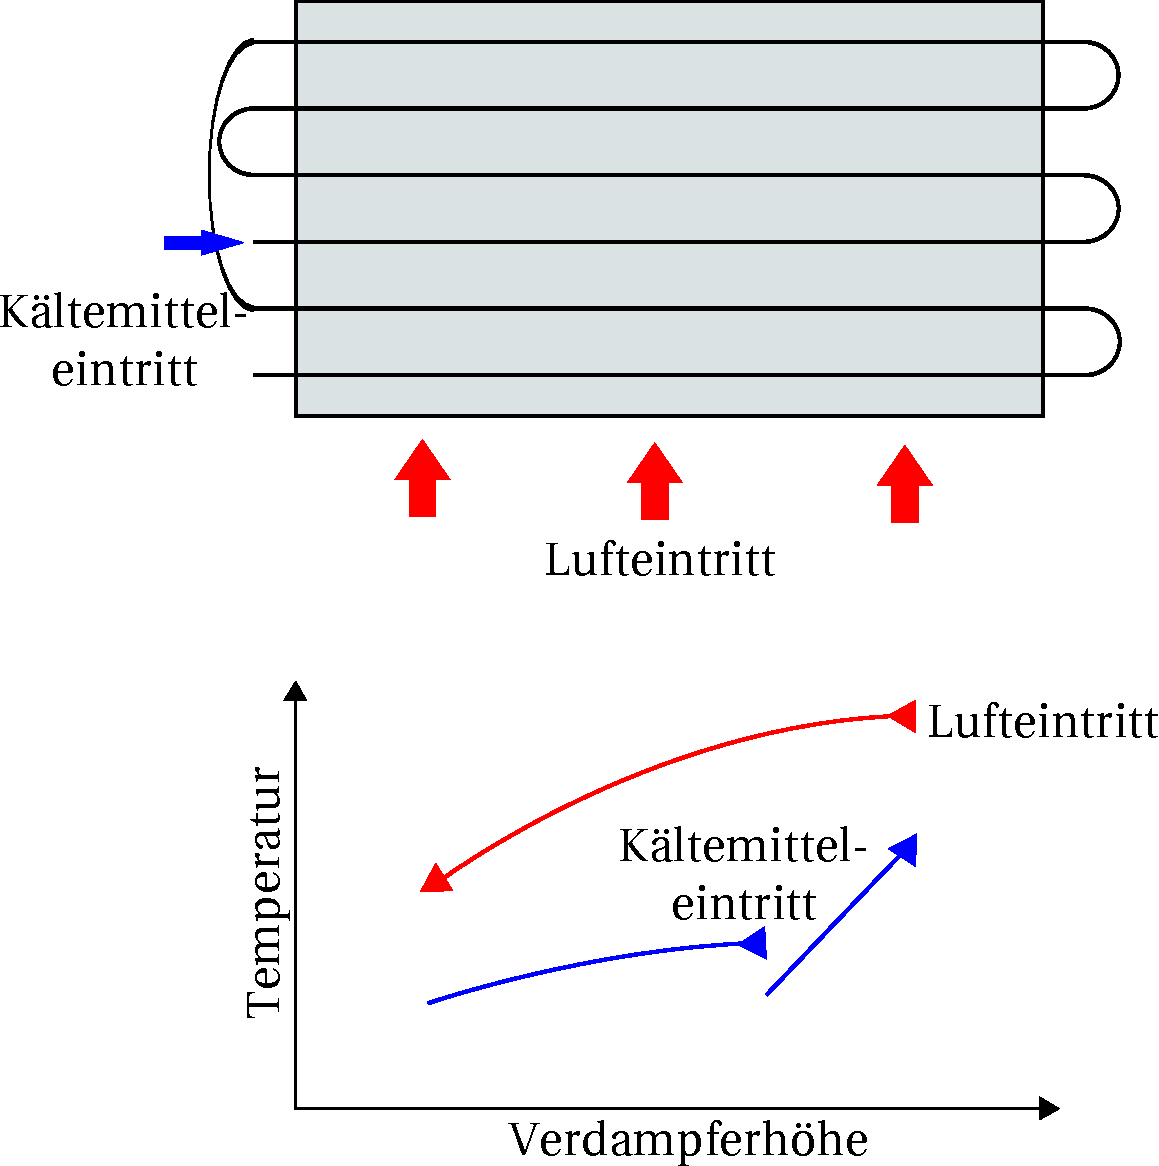
\includegraphics[scale=0.4]{Pictures/Verdampfer_Gleich-Gegenstrom.pdf}}
\caption{Vergleich der Verdampferschaltungen}
\label{fig:Vergleich der Verdampferschaltungen}
\end{figure}


\subsection{Modellierung mit EES}
\label{subsec:Modellierung mit EES}

EES ist ein Gleichungslöser, der es erlaubt Gleichungen mit Unbekannten unabhängig ihrer Reihenfolge effizient zu lösen. Zudem besitzt EES eine Vielfalt integrierter mathematischer, sowie thermodynamischer und physikalischer Funktionen auf die sich bequem zugreifen lässt\cite{Klein.2000}. Ausschlaggebend für den Entscheid über die Nutzung des Programms ist vorallem die integrierte Stoffdatenbank, welche den Zugriff auf die Daten einer Vielzahl von idealen sowie realen Fluiden erlaubt. Eine objektorientierte Modellierung ist leider nicht ohne Weiteres möglich, wodurch der Entwicklungsaufwand stark erhöht wird. Damit das Programm genaue Ergebnisse liefert ist es nötig, physikalisch sinnvolle und und möglichst genaue Begrenzungen der erstellten Variablen anzugeben. 
Weitere Programmfunktionen erlauben die Erstellung einer Benutzeroberfläche sowie die Erstellung von Tabellen und Graphen. Als sehr nützlich erweist sich dabei die Möglichkeit Stoff-Eigenschaftsdiagramme wie z.B. Mollier- oder log-p-h-Diagramme zu erstellen.



\subsection{Berechnung des Druckabfalls in der Zweiphasen-Strömung}
\label{subsec:Berechnung des Druckabfalls in der Zweiphasen-Strömung}

Die Ausgangsberechnung auf der alle weiteren Berechnung basieren, ist die des Druckabfalls innerhalb der Kältemittelströmung.
Der gesamte Druckabfall setzt sich aus einem Reibungsanteil, einem Beschleunigungsanteil und einem statischen Anteil zusammen\cite{SpringerVerlagGmbH.2013}:

\begin{equation}
\Delta p =  \Delta p_{Reibung} \pm \Delta p_{statisch} \pm \Delta p_{Beschleunigung}
\end{equation}

Der statische Anteil, sowie der Beschleunigungsanteil sind von einer viel kleineren Dimension und werden deshalb als vernachlässigbar angenommen. Um den durch Reibung bedingten Druckabfall zu berechnen muss zunächst bestimmt werden ob die Gasphase dispers oder kontinuierlich ist, d.h. ob Gasblasen getrennt und verteilt in der Flüssigkeit transportiert werden oder zusammenhängend strömen.

\begin{equation}
\Delta p_{Reibung} = \int_{l_1}^{l_2} \left( \frac{dp}{dl} \right)_{Reibung} dl
\end{equation}


Die Gasphase ist dispers, wenn gilt:

\begin{equation}
\frac{1}{\beta} = \frac{\dot{V_G}}{\dot{V_L}} = \frac{x\rho_F}{(1-\dot{x})\rho_D} \leq \frac{12\sqrt{Fr}}{1+\frac{\sqrt{Fr}}{7}}
\end{equation}

und als kontinuierlich, wenn gilt:

\begin{equation}
\frac{1}{\beta} = \frac{\dot{V_G}}{\dot{V_L}} = \frac{x\rho_F}{(1-\dot{x})\rho_D} > \frac{12\sqrt{Fr}}{1+\frac{\sqrt{Fr}}{7}}
\end{equation}

In allen durchgeführten Berechnungen ist die Dampfphase als kontinuierlich zu betrachten, daher wird sich im Rahmen dieser Ausführungen auf die Gleichungen dieser Annahme beschränkt. Der Reibungsdruckabfall wird wesentlich durch einen intensiven Impulsaustausch zwischen den beiden Phasen beeinflusst. In den Gleichungen wird die Zweiphasenströmung wie eine Dampfströmung behandelt und der Einfluss der flüssigen Phase durch eine Korrekturgröße $\gamma$ berücksichtigt:

\begin{equation}
\left( \frac{dp}{dl} \right)_{Reibung} = \xi_D \frac{\dot{m}^2 x^2}{4\rho_D} \left(\frac{1}{1-\gamma} \right)^2
\end{equation}

Dabei ist $\xi_D$ der Reibungsbeiwert:

\begin{equation}
\frac{1}{\xi_D} = 2\log(Re_D \sqrt{\xi_D})-0.8
\end{equation}

mit der Reynoldszahl der dampfförmigen Phase:

\begin{equation}
Re_D = \frac{\dot{m} x d}{\eta_D}
\end{equation}

Die Korrekturgröße $\gamma$ ist als effektive Querschnittsverengung für den Dampfstrom, verursacht durch die Flüssigkeit, zu interpretieren und kann als Versperrungsfaktor bezeichnet werden. Abhängig von den Geschwindigkeiten und den Dichteverhältnissen muss abschnittsweise zwischen verschiedenen Strömungsformen unterschieden werden. Bei kleinen Massenstromdichten ist die Strömung eben und geschichtet. Bei gesteigertem Durchsatz wird sie wellig und es treten Schwalle auf, durch die der Rohrumfang vollständig von Flüssigkeit benetzt ist. Bei noch höheren Durchsätzen wird die Flüssigkeit tropfenförmig im Gaskern mitgerissen. Durch erhebliche Expansionseffekte bei hohen Geschwindigkeiten findet eine Beschleunigung der Dampfphase statt und es stellt sich ein Schlupf zwischen den beiden Phasen ein\cite{Kesper.1976}.

\begin{equation}
\gamma = \gamma_F(1-E) + \gamma_E E
\end{equation}

Hierbei ist der Verperrungsfaktor für ebene Strömung:

\begin{equation}
\gamma_E = 1 - \left( 1+0.15 \left( \frac{1-x}{x} \right)^{0.45} \left( \frac{\eta_f}{\eta_D}-1 \right)^{0.25} (1 + 3x^4)\right)^{-1}
\end{equation}

der Versperrungsfaktor für Ringströmung mit Schwallen:

\begin{equation}
\gamma_F = 1 - \left(1+\frac{(1-x)\rho_D}{x \epsilon \rho_F}\right)^{-1.19}
\end{equation}


und $E$ ein Verteilparameter:

\begin{equation}
E = 1.857 + 0.815 \log\left[\left(\frac{\dot{m} x}{\rho_D c_G}\right)^2 \left( 1+ \frac{4575 \rho_D^2}{\rho_F^2} \right)\right]
\end{equation}

$E$ darf immer nur Werte zwischen 0 und 1 annehmen. Liegt ein Ergebnis außerhalb dieses Bereichs wird E mithilfe einer Bedingung auf 0 bzw. 1 gesetzt. Bei $E=0$ ist die Strömungsform Ringschwallströmung, bei $E=1$ beschleunigte Strömung.
Für die Berechnung von $\gamma_F$ ist außerdem die Berechnung der Hilfsgrößen $\epsilon$ und $\psi$ nötig:

\begin{equation}
\epsilon^{-3} = \epsilon_1^{-3} + \epsilon_2^{-3}
\end{equation}

mit

\begin{equation}
\epsilon_1 = 1.71 \psi^{0.2} \left( \frac{1-x}{x} \right)^{0.15} \left( \frac{\rho_D}{\rho_F} \right)^{0.5} \left( \frac{\eta_D}{\eta_F} \right)^{0.1}
\end{equation}

und

\begin{equation}
\epsilon_2 = 9.1 \psi
\end{equation}

sowie

\begin{equation}
\psi = (Re_F Fr_F)^{-\frac{1}{6}} \left( \frac{1-x}{x} \right) \left(\frac{\rho_F}{\rho_D} \right)^{-0.9} \left(\frac{\eta_F}{\eta_D} \right)^{-0.5}
\end{equation}

\subsection{Berechnung des Wärmeübergangs}
\label{subsec:Berechnung des Wärmeübergangs}

Die Ausgangsgröße der Temperatur von Luft und Kältemittel nach jeder Zelle wurde mittels der $\epsilon-NTU$-Methode berechnet\cite{SpringerVerlagGmbH.2013}\cite{Bergman.2011}\cite{Nellis.2009}. $NTU$ (dt. Anzahl der Übertragungseinheiten) und $\epsilon$ bezeichnen dimensionslose Kennzahlen. Diese Methode ist ein Verfahren, das oft bei der Auslegung von Wärmetauschern verwendet wird, da es teils schwierige Berechnungsschritte erspart. Zunächst ist es erforderlich die Wärmekapazitätsströme der beiden Fluide zu bestimmen. Für den Wärmekapazitätsstrom der Luft gilt:

\begin{equation}
\dot{C}_{min} = \dot{m}_h c_{p,h}
\end{equation} 

Für den Wärmekapazitätsstrom des Kältemittels gilt:

\begin{equation}
\dot{C}_{max} = \dot{m}_k c_{p,k}
\end{equation}
 
Das Wärmekapazitätsverhältnis $C_r$ ist damit:
 
\begin{equation}
C_r = \frac{\dot{C}_{min}}{\dot{C}_{max}}
\end{equation}

Zudem ist es notwendig den Wärmedurchgangskoeffizienten $U$ zu berechnen\cite{LehrstuhlfurWarmeundStoffubertragung.}. Dieser setzt sich aus den Wärmeleitwiderständen der einzelnen Rohrschichten und Übergängen zusammen. Um flexibel bei der Anpassung der Parameter des Modells an die Realität zu sein wurde hierbei auf eine Analogie zu Widerständen in Reihenschaltung aus der Elektrotechnik zurückgegriffen und die wärmeübertragende Fläche $A$ direkt mit einbezogen. Somit ist:

\begin{equation}
UA = \frac{1}{R_{L} + R_{Al} + R_{Cu} + R_{Km}}
\end{equation}
 
samt der einzelnen Wärmeleitwiderstände:

\begin{equation}
R_L = \frac{1}{\alpha_{L} d_{Al} \pi l}
\end{equation}

\begin{equation}
R_{Al} = \frac{t_{Al}}{\lambda_{Al} d_{Al} \pi l}
\end{equation}

\begin{equation}
R_{Cu} = \frac{t_{Cu}}{\lambda_{Cu} d_{Cu} \pi l}
\end{equation}

\begin{equation}
R_{Km} = \frac{1}{\alpha_{Km} d_{i} \pi l}
\end{equation}

Die Rohrgeometrie ist dabei wie in Abbildung~\ref{fig:Geometrie} dargestellt.
Die Wärmeübergangszahlen wurden mit Orientierung am realen Modell bestimmt. Näheres dazu in Kapitel~\ref{cha:Durchgeführte Untersuchungen}.

\begin{figure}[h]
\centering
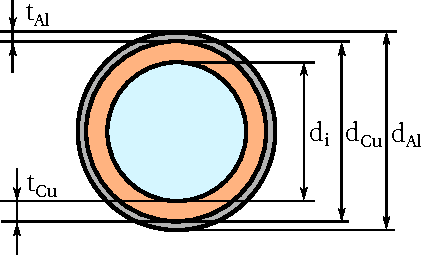
\includegraphics[scale=1]{Pictures/Rohrgeometrie.pdf}
\caption{Geometrie des Verdampferrohres}
\label{fig:Geometrie}
\end{figure}

Mit diesen Größen lässt sich nun der $NTU$-Wert berechnen:

\begin{equation}
NTU = \frac{UA}{\dot{C}_{min}}
\end{equation}

Damit lässt sich nun die Effektivität des Wärmeübertragers $\epsilon$ bestimmen.
Dabei muss zwischen sensibler und latenter Wärmeaufnahme des Fluids unterschieden werden.
Findet ein Verdampfungsprozess statt so gilt $C_{max}\longrightarrow\infty$ und damit $C_r =0$. Für diesen Fall gilt:

\begin{equation}
\epsilon = 1- exp{-NTU}
\end{equation}

Für den Fall überhitzenden Kältemittels und reinem Kreuzstrom gilt:

\begin{equation}
\epsilon = 1- exp{\left[\left(\frac{1}{C_r}\right)(NTU)^{0.22}(exp{[-C_r(NTU)^{0.78}]}-1)\right]}
\end{equation}

Mit diesen Größen ist es nun möglich den übertragenen Wärmestrom zu berechnen:

\begin{equation}
\dot{Q} = \epsilon \dot{C}_{min} (T_{L,ein} - T_{Km,ein})
\end{equation}

Hierbei ist die Eintrittstemperatur des Kältemittels die Sättigungstemperatur bei Eingangsdruck. Aus der Energiebilanz lassen sich dann Kältemittelaustrittsenthalpie sowie Luftaustrittstemperatur bestimmen:

\begin{equation}
\dot{Q} = \dot{M}_{Km} (h_{Km,ein} - h_{Km,aus}) = \dot{M}_{L} c_{p,L}(T_{L,ein} - T_{L,aus})
\end{equation}





\subsection{Das Modell}
\label{subsec:Das Modell}

Mithilfe der in Abschnitt~\ref{subsec:Berechnung des Druckabfalls in der Zweiphasen-Strömung} und \ref{subsec:Berechnung des Wärmeübergangs} vorgestellten Gleichungssysteme lassen sich, durch Angabe der Eingangswerte Druck, Dampfanteil, Temperatur und Massenstrom des Kältemittels sowie Temperatur und Massenstrom der Luft, Ausgangswerte nach einer definierten Rohrlänge berechnen. Da die Ergebnisse innerhalb einer Zelle allein von den Eingangswerten abhängig sind bietet eine Unterteilung in mehrere kleine Zellen eine viel höhere Genauigkeit. Um Rechenaufwand und Genauigkeit in der Waage zu halten und mit Orientierung am realen Verdampfer wird das Modell entsprechend der Anzahl der Verdampferrohre eines Kältemittelkreises mittels der Zellenmethode in sechs Berechnungszellen unterteilt\cite{LehrstuhlfurWarmeundStoffubertragung.b}.
Über die Benutzeroberfläche lässt sich der Zustand beider Fluide nach jeder einzelnen Zelle observieren und somit direkt mit den Daten des realen Verdampfers vergleichen.
Das Modell ist nur gültig für die Annahme trockener Luft. Da auch in einer Klimakammer \unit{0}{\%} relative Feuchtigkeit schwierig zu erreichen sind, ist eine Abweichung der Ergebnisse zu erwarten.




\begin{figure}[htb]
\centering
	\subfigure[Gleichstrom]{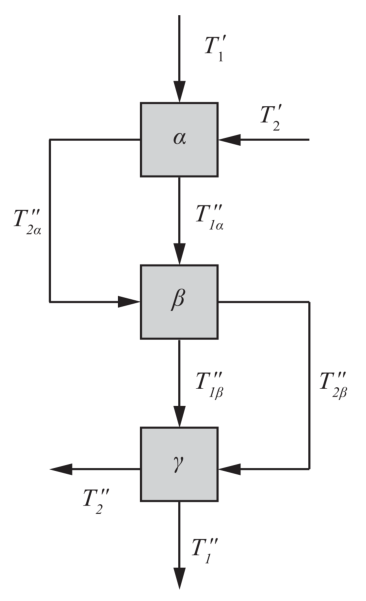
\includegraphics[scale=1]{Pictures/Zellenmethode_Gleichstrom.pdf}}
	\subfigure[Gegenstrom]{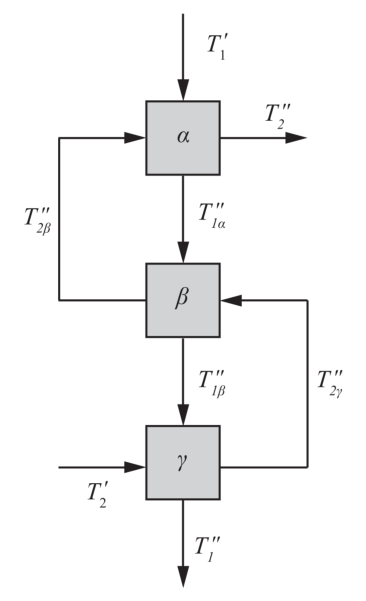
\includegraphics[scale=1]{Pictures/Zellenmethode_Gegenstrom.pdf}}
\caption{Zellenmethode}
\label{fig:Zellenmethode}
\end{figure}